\chapter{Comparison To Other Solutions}
\label{chap:comparisontoothersolutions}

\section{Goal Oriented Action Planning}
\label{sec:comparisontoothersolutions_goalorientedactionplanning}

With Goal Oriented Action Planning (GOAP), the agent is able to plan the best sequence of actions, depending on the current state of the environment, to achieve a given goal as efficiently as possible. It can generate different action plans, evaluate their costs, and then choose the one that best fits the current circumstances. Every plan can consist of several actions, each associated with a weight to help the agent decide on the best sequence. \cite{GOAP}

A good example is the goal for an agent to get apples. Suppose there are three actions the agent could perform: pick the apple, grab ladder and buy apples. To perform the action of picking an apple, the agent first needs a ladder, otherwise the apple is out of reach. The actions can be given an individual cost:

\begin{tabular}{lp{12cm}}
pick apples: & 3 cost \cr
grab ladder: & 4 cost \cr
buy apples: & 8 cost
\end{tabular}

Now there are two different sequences of actions that the agent can choose from to achieve his goal of getting apples:

\begin{tabular}{lp{12cm}}
grab ladder -> pick apples: & total cost: 7 \cr
buy apples: & total cost: 8
\end{tabular}

Because the sequence of actions of grabbing his ladder and then picking apples has a lower cost than buying apples, it would choose that sequence. However, if the cost of the ladder increases because the ladder is broken and the agent would have to fix it first, then it might decide to just go and buy some apples because the cost of doing so is lower.

Also, the agent could learn a new skill that allows him to climb trees at a cost of only 2. With GOAP, this new action could then simply be added to the other actions, and the framework would take it into account when making decisions. As a result, the agent would never need to use the ladder again.
In order for the framework to plan its actions, each action must have preconditions and effects. Similar to utility AI, preconditions must be met for an action to be executed. Effects, on the other hand, are NOT the executed behaviour, they only represent the state that would be achieved if this action were executed. Effects are only used by the GOAP planner to plan ahead. As an example, the actions could have the following preconditions and effects, where "has apples" is the goal:

\begin{tabular}{lp{12cm}}
pick apples: & Preconditions: "in range to pick" | Effect: "has apples" \cr
grab ladder: & Preconditions: "ladder available", "doesn't have ladder" | Effect: "in range to pick" \cr
buy apples: & Preconditions: "shop is open" | Effect: "has apples"
\end{tabular}

\newpage

With this information, the GOAP planner can now iterate through all possible sequences of actions to find the path with the lowest cost. It will also look at sequences that don't make much sense, like "grab ladder" -> "buy apples". But since the cost is too high with (4 + 8) = 12, it will not be chosen. Buying apples directly is always cheaper. \cite{GOAP}

This solution is closest to utility AI because it's also able to react intelligently without having to script every possible situation, resulting in more dynamic behaviour. The GOAP cost system is analogous to the utility AI score system. The main difference is that GOAP is goal based and creates an optimal sequence of actions and then executes them one by one. Utility AI, on the other hand, will always choose the action that best suits the current situation, without making a plan for the next actions. Depending on the implementation, there may be other differences, such as how costs and points are calculated. Also, the way information from the world is evaluated with curves in utility AI may be different when using GOAP.

\section{Reinforcement Learning}
\label{sec:comparisontoothersolutions_reinforcementlearning}

Reinforcement learning (RL) is a machine learning model where the agent can learn from an interactive world by trying and learning from the outcome. With RL, the programmer no longer needs to specify the weights for how important which action is. Instead the agent will figure it out by trying different approaches and then getting rewarded or punished for the outcome. \cite{RL}

Reinforcement Learning is a machine learning model where the agent can learn from an interactive world by trying and learning from the result. With RL, the programmer no longer needs to specify weights for how important an action is. Instead, the agent figures it out by trying different approaches and then being rewarded or punished for the outcome.

\newpage

\section{Overview Of All Solutions}
\label{sec:comparisontoothersolutions_overviewofallsolutions}

\begin{figure}[H]
	\centering
		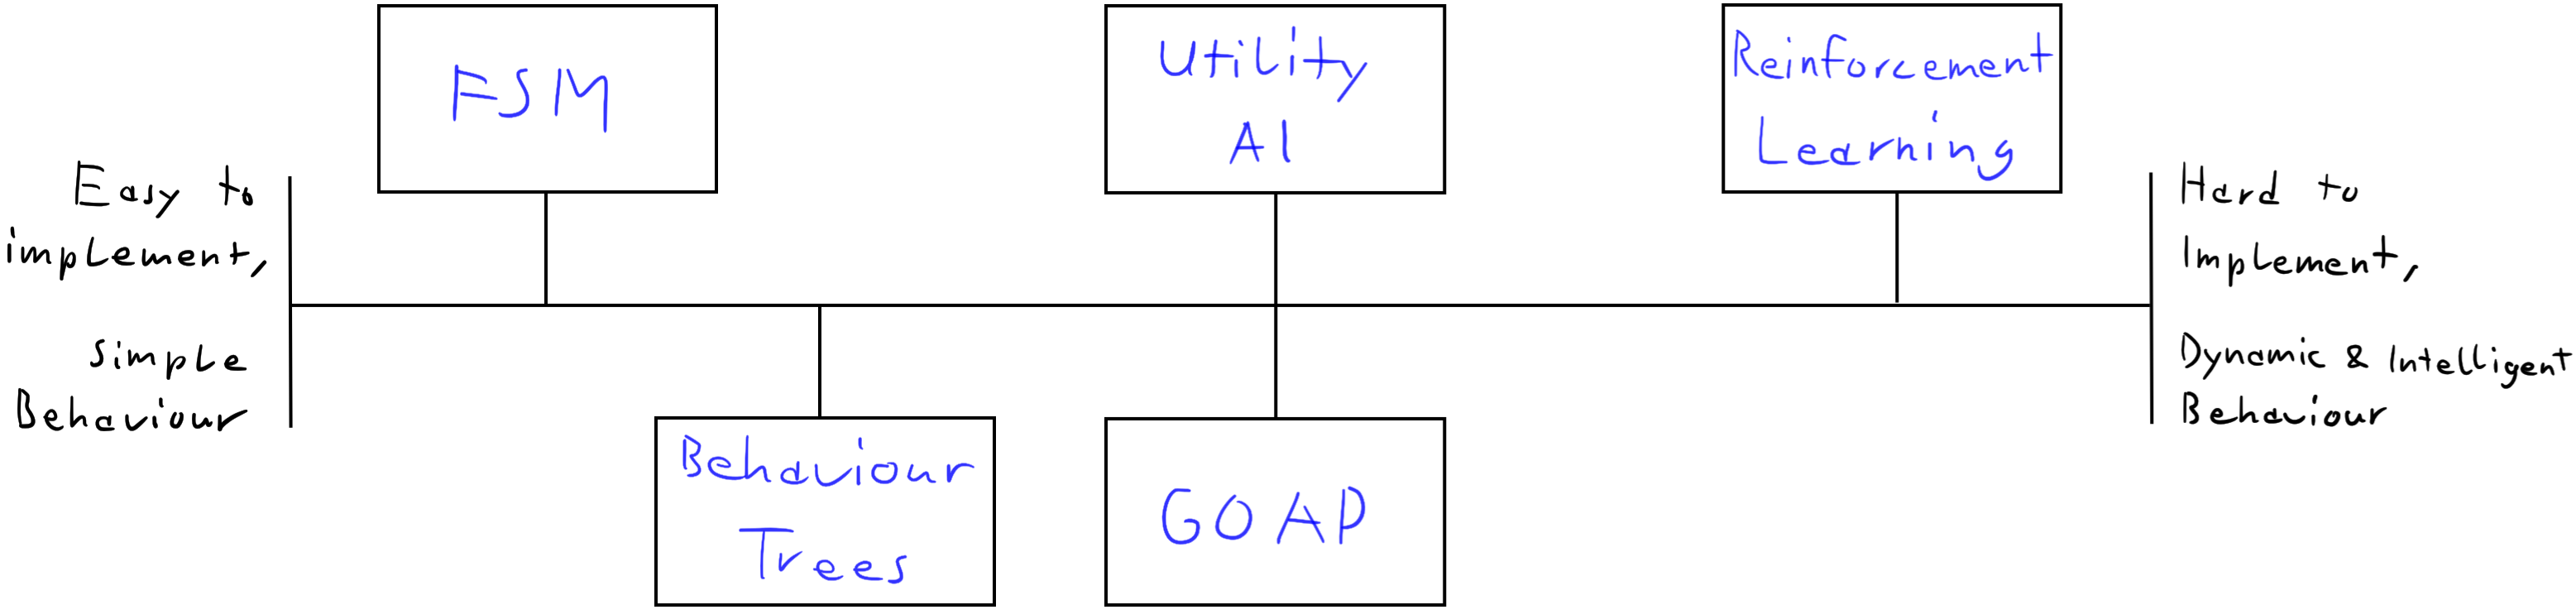
\includegraphics[scale=0.19]{images/comparison_of_ai_solutions.png}
	\caption{Comparison of solutions used for NPCs \cite{Comparison}}
	\label{fig:comparison_of_ai_solutions}
\end{figure}

This sketch shows all the solutions presented in this paper, from those that are easy to implement and understand, to those that are more complex but will result in more intelligent behaviour. There is no "best solution" for every situation. Depending on the problem, the right solution needs to be chosen, and utility AI is just one of them.

The requirements for an NPC depend very much on how complex it needs to be, and what kind of behaviour is required. For a very simple scenario, an FSM might be just fine, and it's also very easy to implement. But for more complex behaviours, it's often worth the time to learn or even implement a more complex solution.

A developer must also consider the performance of the application. If you have a game with hundreds of zombies running towards the player, it might be too expensive to give each one the ability to decide the best sequence of actions using, for example, GOAP. It would also take more time to implement, and on top of all, the player might not even notice the intelligence of the enemies because they are too many and die with a few shots anyway.